\documentclass[a4paper,12pt]{article}

\usepackage[utf8]{inputenc}
\usepackage[ngerman]{babel}
\usepackage[T1]{fontenc}
\usepackage{graphicx}
\usepackage[cache=false]{minted}
\usepackage{dirtree}

\begin{document}
\begin{titlepage}
    \begin{center}
        \vspace*{1cm}
        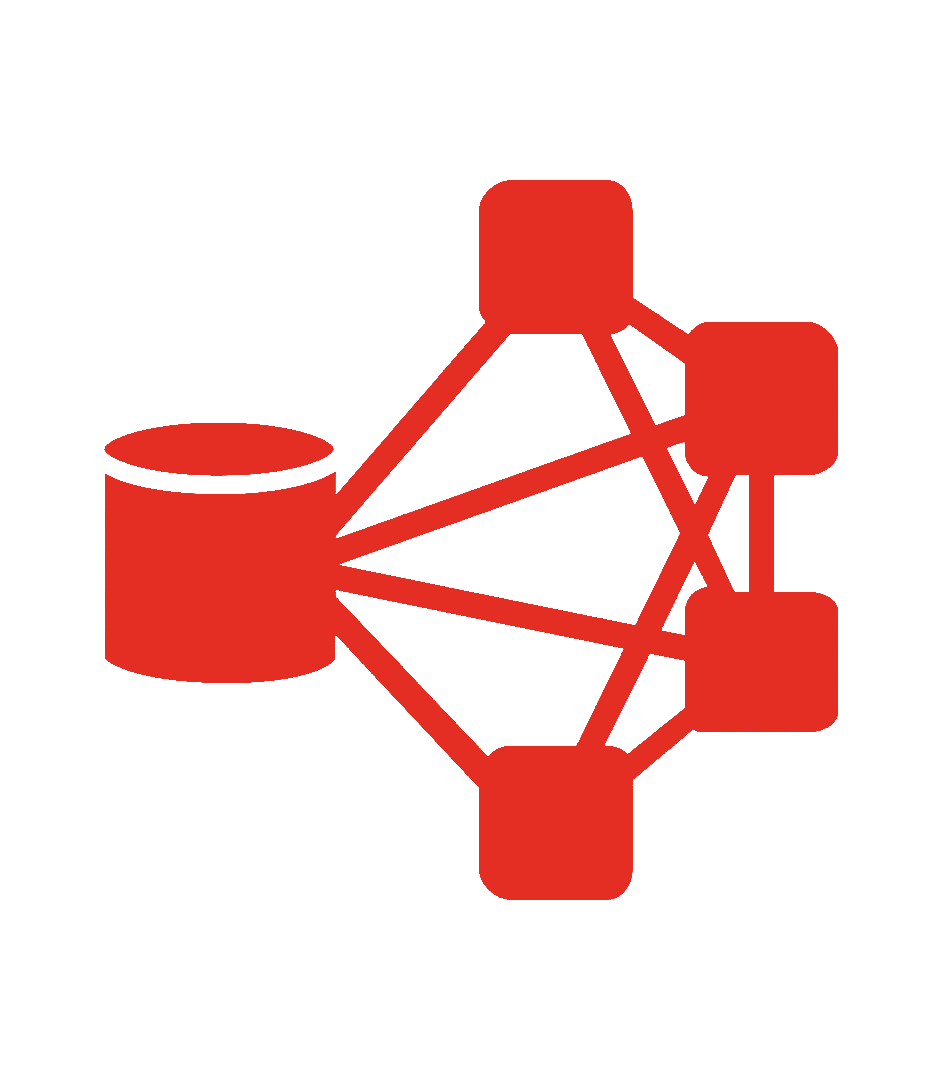
\includegraphics[width=10cm]{Logo.png}
        
        \textbf{\huge MapReduce-System}
        
        \vspace{0.5cm}
        NVS Projekt 2
                 
        \vspace{1.0cm}
    
        \textbf{Alexander Grill 5CHIF}
        
        \today
        
        \vfill
                 
                 
        \vspace{0.5cm}
                 
        Informatik\\
        HTBLUvA Wr.Neustadt\\
        Österreich\\

                 
    \end{center}
\end{titlepage}  
\newpage
\tableofcontents
\newpage


\section{Einführung}

\subsection{Vorwort}

\subsection{Motivation}

\section{Aufgabenstelllung}

\subsection{Erläuterung der Grundproblematik}

\subsection{Idee}

\subsection{Themenbereiche}
\newpage
\section{Grundlagen}

\subsection{Was ist ein MapReduce System?}
Das Verfahren wurde 2004 von Google entwickelt für die Indexierung von Webseiten. Das Framework wird bei Datenbanken eingesetzt und dient zur Verarbeitung von großen, komplexen, unstrukturierte Datenmengen.
Dieses Verfahren findet Anwendung für BigData und Datawarehouse, weil in solchen Fällen große Datenmengen in kürzester Zeit mittels Software verarbeitet, analysiert, aggregiert als auch kompremiert werden. 
Map Reduce parallelisiert die Bearbeitung, durch die Verteilung auf mehrere gleichzeitig auszuführende Tasks. Der Grund, warum dieses Framework solche Datenmengen verarbeiten kann ist, weil die Aufgaben auf mehreren Rechnern aufgeteilt werden. Jeder einzelne Rechner startet Prozesse, die Parallel die Daten verarbeitet und auswertet.
Ein einzelner Rechner stoßt schnell an seine Grenzen, deshalb ist die Verarbeitung von Daten, mittels mehreren Knoten sehr effizient und bietet eine bessere Performance.
Das Verfahren wurde in vielen verschiedenen Verfahren eingesetzt wie zum Beispiel für die Indizierung von Webseiten, nach einer Suchanfrage mit beliebigen Zeichenketten, ebenso im Umfeld von Google News wird MapReduce verwendet. Andere große Internetfirmen wie Yahoo, die ebenfalls das Verfahren für die Indexierung von Webseiten verwenden, 
als auch Facebook verwendet das System, um Spam Messages zu minimierung und die Ads zu optimieren. Wohingegen Amazon das Verfahren für das Clustering der Produket verwendet

\subsection{Map und Reduce}
Die beiden Grundfunktionen des Verfahrens sind Map und Reduce. Sie sorgen für die Aufteilung der Aufgaben in kleinere parallelisierten Arbeitspakete und führen am Ende die Ergebnisse zusammen. Bei großen relationalen Datenbanken und komplexen Queries lassen sich typische Problem, bezglüch Verarbeitung von großen Datenmengen beseitigen.
Die Map Funktion, verteilt die Aufgaben an unterschiedlichen Knoten eines Clusters. Die Reduce Funktion sortier die verfassten Ergebnisse und fügt sie am Ende wieder zusammen.
Die Funktionen Map und Reduce werden vom User bereitgestellt, weil diese schließlich zu den bereitgestellten Daten passen müssen.
\newpage

\subsection{Ablauf}

\begin{figure}[h]
    \centering
    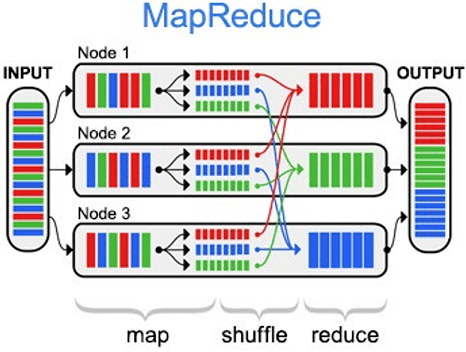
\includegraphics[width=6.1cm]{mapreduce.png}
\end{figure}

\begin{description}
    \item[Das Verfahren verläuft durch folgende Schritte:] ~\par
    \begin{itemize}
        \item Split
        \begin{itemize}
            \item{Die bereitgestellten Daten werden aufgeteilt. Jeder Datensatz darin ist identifiziert durch
            einen Schlüssel-Wert. Diese Datenmenge wird nun in kleinere Datenmengen aufgeteilt
            und vom Master an die verfügbaren Knoten verteilt.}
        \end{itemize}
        \item Map 
        \begin{itemize}
            \item{Nun wendet jeder Knoten auf die Daten die Map-Funktion an, die schließlich Key/Value Paare zurückgibt. Diese Ergebnisse werden zwischengespeichert.}
        \end{itemize}
        \item Shuffel
        \begin{itemize}
            \item{Bei diesem Schritt geht es darum den reduce-Knoten, die entsprechenden Daten zuzuteilen.
            Diese Zuteilung entspricht einer Fragmentierung.
            Hierbei wird den Knoten, die reduce ausführen, ein Key zugeteilt. Diese Knoten holen sich
            dann die bereits durch Map entstandenen Datensätze mit diesem Key und wenden reduce an.}
        \end{itemize}
        \item Reduce
        \begin{itemize}
            \item{Grundsätzlich ist die Aufgabe dieser Funktion, die Key/Value Paare anhand des Schlüssels
            zusammenzufassen und dabei die Summe der einzelnen Values zu bilden. Demnach ist die
            Ausgabe der Reduce-Funktion wieder ein Key/Value Paar mit dem gleichen Aufbau wie vor
            der Verarbeitung.
            Dies ermöglicht es, dass reduce mehrere Male angewendet werden kann, bis schließlich alle
            Daten gesammelt wurden.}
        \end{itemize}
    \end{itemize} 
\end{description}





\section{Umsetzung}

\subsection{Aufbau}

\subsection{Klassendesign}

\subsection{Source Code Dokumentation}

\subsection{Verwendete Bibliotheken}

\section{Anwendungsfälle}

\section{Schlusswort}

\end{document}
